\section{Hardware Choice} \label{Hardwarechoice}
From the prototype description, see \secref{Finalprototype} it is possible to choose compatible hardware for building the prototype. 
Some of the hardware components are given with the vehicle, see \secref{sec:Vehicledescription}, and therefore, are not described in this section. 
The availability of the components and their compatibility with the system also have to be considered.

%%%%%%%%%%%%%%%%%%%%%%%%%%%%%%%%%%%%%%%%%%%%%%%%%%%%%

\subsection{Microcontroller}
The microcontroller is utilized to control the system and the connected hardware. Thus containing software used for controlling the system by sending and receiving electrical signals as needed.

Requirements for the microcontroller:
\begin{itemize}
% \item Having a CPU, that has a frequency greater than \si{XX\ MHz}. \todo{Number}
\item Having I/O connections, both digital and analogue, see \secref{sec:Vehicledescription}.
\item Having output connections, that can transmit PWM signals, see \secref{sec:Vehicledescription}.
\item Having 5 free timers. Two for the Hall sensors and one for the kernel, motor, servo-motor.
%\item Being powered by an external power source, thereby being able to .
\end{itemize}

\subsubsection{Arduino Mega 2560}
The Arduino Mega 2560 is a microcontroller board, which comes with an 8-bit ATmega2560 integrated circuit and extends its I/O ports, see \figref{ArduinoMega} \cite{MegaInfo}. 

\begin{figure}[H]
	\centering
	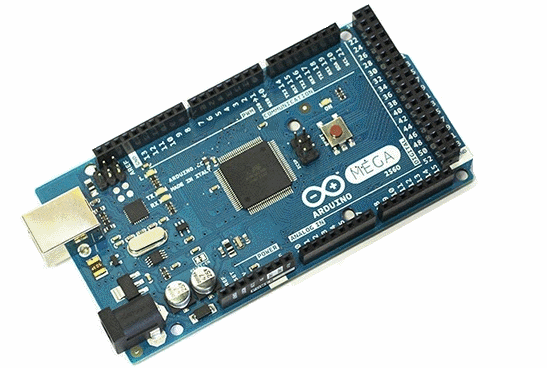
\includegraphics[width=0.5\textwidth]{figures/ArduinoMega.png}
		\caption{An Arduino Mega 2560 board \cite{MegaInfo}} 
	\label{ArduinoMega}
\end{figure}
%
The Arduino Mega has \si{54} digital ports with a 5 volts logic. From these, \si{15} can be used to generate PWM signals. The CPU runs at \si{16 MHz} and the chip has \si{6} integrated timers, one of which is used by the Arduino itself. There are also 4 UARTs, used in serial communication, as well as a setup for SPI communication and an \si{I^2C} bus. The Arduino can be powered though a USB cable or with an external power source.

The Arduino Mega board has been chosen as the microcontroller utilized. The reason is that the connections needed are available. Furthermore, it is possible to find a lot of helpful documentation on the Arduino Mega on the internet. The Arduino is programmable through a serial connection, with the help of avrdude\cite{Avrdude} or simply through the Arduino IDE\cite{ArduinoIDE}. The IDE can compile C, C++ and Arduino (syntax very close to C and C++) files.

%%%%%%%%%%%%%%%%%%%-STORAGE-%%%%%%%%%%%%%%%%%%%%%%

\subsection{Storage}
The storage is used for saving the predetermined route for the vehicle see \secref{Finalprototype}.

An approximation of the needed storage size for the mowing route is made by considering, a lawn of \si{10\ m} by \si{10\ m} and a simple path with parallel lines which require two points each. Since a route point is defined by two coordinates x and y of size \si{4\ B} in total, and the vehicle is \si{29\ cm} wide, see \secref{sec:Vehicledescription}, the storage capacity is approximated to:
\begin{flalign}
	\eq{Capacity}{\frac{10}{0.29} \cdot 2 \cdot 2 \approx 276\ B}
\end{flalign}
This allows to store data points for the lawn mower to cover the whole area without overlapping and with a very simple route. Since this is only a rough calculation, a SD card with a capacity of more than this should be chosen for containment of a predetermined route. Furthermore it would be practical to utilize the SD card when testing. Therefore a SD card with a capacity of at least 1 GB should be chosen.

To find an estimate of the required storage transfer rate when retrieving data, the steering control requirements in terms of sampling frequency are considered, this is found in \secref{sec:steeringController}, as this utilizes the route coordinates. Since the servomotor needs to receive data every \si{30\ ms} \cite{futaba}, the receiving of data from storage needs to be done in the meantime. The other tasks also needs a certain time to run. This time can be approximated to \si{2\ ms}, see \secref{sec:scheduling}, and has to be substracted from the \si{30\ ms}. Furthermore, the data transfer during each turn should not take too much time, and it is arbitrary decided to take a tenth of the available time. As each point weighs \si{2\ B}, the minimum transfer rate needed is:
\begin{flalign}
	\eq{Transfer\ rate}{\frac{1}{\frac{0,030 - 0,002}{10}} \cdot 2 \approx 714,3\ B = 7,2 B \cdot s^{-1}}
\end{flalign}

Requirements for the storage:
\begin{itemize}
\item Offering the possibility to retrieve the data after a power cut to the storage.
\item Having a storage of at least \si{1 GB}. 
\item Having a transfer speed greater than \si{7,2}\si{KB \cdot s^{-1}}.
\end{itemize}

\subsubsection{SD Card} \label{SDcard}
Secure Digital (SD) card is a type of non-volatile flash memory cards. This means that the data will not be lost during a power cut off.

It comes in various storage sizes, from 1 GB to 2 TB, depending on which type of SD card it is\cite{SDassociation}. There is 3 types of SD card, the standard capacity (SDSC), the high capacity (SDHC) and the extended capacity (SDXC). The difference between the different types, is the file system utilized on the card and their maximum capacity. With the requirement of a storage size on 1 GB bytes, and a desired need for utilizing it to the contain test data, a SDSC with a capacity of 2 GB is chosen.

The lowest transfer speed for an SDSC card is \si{2 MB/s}\cite{SDassociation}. With the requirement of a transfer speed greater than si{7,2}\si{KB \cdot s^{-1}}, makes the SDSC card fast enough. 

To use the SDSC card and connect it to the microcontroller, 7 connection pins are required, see \figref{SDcardpinout}. The setup of the SD card is different, depended on which mode is used.

\begin{minipage}{\linewidth}
      \centering
      \begin{minipage}{0.65\linewidth}
			\begin{table} [H]
				\begin{tabular}{|l|l|l|l|}
								
\hline
\textbf{Pin} & \textbf{SPI}  		& \textbf{One bit} 	& 	\textbf{Four bit}  \\
\hline
1			 &	Unused		 		&	Unused			    &	Data 2			   \\
\hline
2			 &	Card Select	 		&	Card Detection		&	Data 3			   \\
\hline
3			 &	Data In		 		&	\begin{tabular}{@{}l@{}} Command \&  \\Response \end{tabular}  &	\begin{tabular}{@{}l@{}} Command \&  \\Response \end{tabular} \\
\hline
4			 &	Power 				&	Power			    &	Power			   \\
\hline
5			 &	Serial clock 		&	Serial clock		&	Serial clock	   \\
\hline
6			 &	Ground		 		&	Ground			    &	Ground			   \\
\hline
7			 &	Data Out	 		&	Data 0			    &	Data 0			   \\
\hline
8			 &	Unused		 		&	Unused			    &	Data 1			   \\
\hline		
				\end{tabular}
				\caption{SD card pinout configuration\cite{elasticsheep}}
				\label{SDcardconf}				
			\end{table}			
      \end{minipage}
      \hspace{0.03\linewidth}
      \begin{minipage}{0.30\linewidth}
          \begin{figure}[H]
              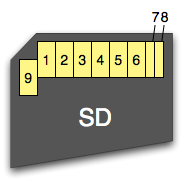
\includegraphics[width=0.95\textwidth]{figures/sdcardpinout}
              \caption{Illustration of a micro size SD card.\cite{elasticsheep}} 
              \label{SDcardpinout}
          \end{figure}
      \end{minipage}
      
  \end{minipage}


The power needed for the SD card is 3.3 volts\cite{elasticsheep}. There are three possible setups for the SD card: SPI, One-Bit and Four-Bit.
With the SPI setup, the communication between the SD card and the microcontroller is made on two lines. With the One-Bit setup, the commands between the SD card and microcontroller are sent on one line and the data is sent through another one.
With the Four-Bit setup, three more data connections are used.

In this project, the SPI setup is used, since the extra transfer speed from the Four-Bit setup is not needed. Furthermore, the Arduino has 4 pins that can be set up to SPI communication\cite{MegaInfo}.

An SDSC card, with a SPI setup is chosen, since this as has a high enough capacity and transfer speed. Furthermore the data is saved, if the power is cut off and the Arduino Mega has SPI connections. 


%%%%%%%%%%%%%%%-Motor Driver-%%%%%%%%%%%%%%%%%%%%

\subsection{Motor Driver}
The motor driver is the connection between the microcontroller, the power supply and the motor. It is used, to isolate the hardware components functioning in low power, i.e. the microcontroller, from the high power parts, i.e. the motor.

The requirements for the motor driver are:
\begin{itemize}
\item Having to be controlled by the microcontroller.
\item Offering the possibility to power it through an external power source.
\item Being able to handle the battery pack's voltage.
\item Allowing to power the motor in both directions.
\end{itemize}

\subsubsection{Pololu Dual VNH5019}
The Pololu dual VHN5019 motor driver shield (see \figref{MotorDrive}) is specially designed for Arduino boards. It can be placed directly on top of the the Arduino board as a shield, with the pins connecting to the right ports on the Arduino.\cite{PCorporation}

\begin{figure}[H]
	\centering
	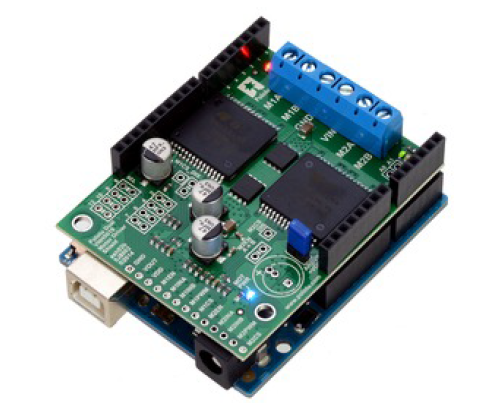
\includegraphics[width=0.50\textwidth]{figures/Motordriver.png}
		\caption{The motor shield on top of an Arduino Uno.\cite{DriverShield}} 
	\label{MotorDrive}
\end{figure}

It is possible to power the Arduino from an external power source through the motor shield, which also delivers the power to the motor. It is also possible to have the motor shield and the Arduino powered separately. This is determined by a jumper setting on the shield, see \figref{MotorDriveIO}. The motor shield need a power voltage between 7 volts and 12 volts.\cite{PCorporation}

\begin{figure}[H]
	\centering
	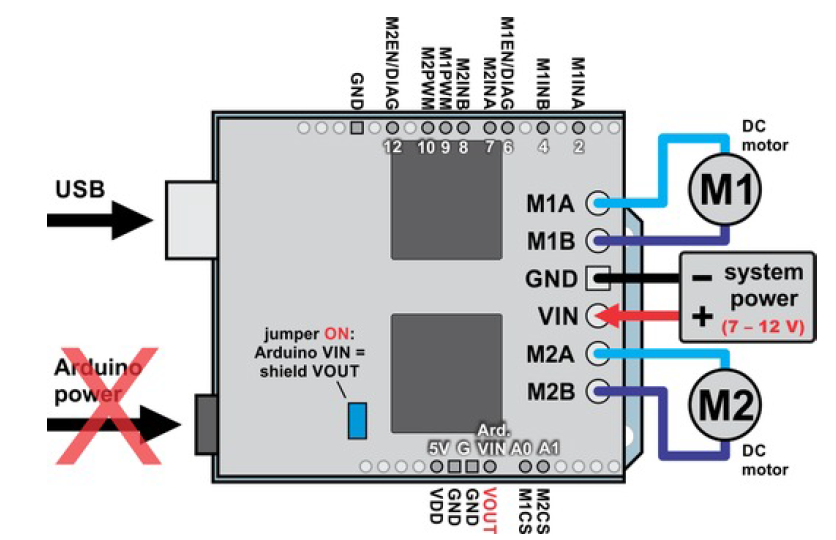
\includegraphics[width=0.60\textwidth]{figures/MotordriverIO.png}
		\caption{Setup for the mort shield.\cite{DriverShield}}
	\label{MotorDriveIO}
\end{figure}

There are two H-bridges on the board, to control up to two motors. Since only one motor is used in this project, both of the two H-bridges will be used to power the motor, see further details on the configuration in \secref{sec:HBridge}. This results in a smaller current through the two H-bridges' transistors and therefore ensures a better protection of the system.\cite{PCorporation}

%\begin{figure}[H]
%	\centering
%	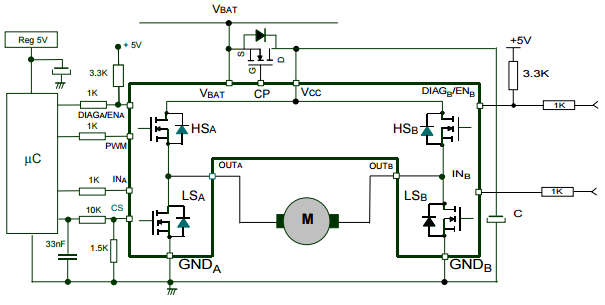
\includegraphics[width=0.85\textwidth]{figures/Hbridges.png}
%		\caption{Illustration of the H-bridge, that the motor shield have two of.}
%	\label{Hbridges}
%\end{figure}
%
The Pololu dual VHN5019 motor driver shield is used in this project, as it is made for the Arduino and therefore easy to implement. Moreover, it can power the Arduino through an external power source and get a power output high enough for the motor and in each direction.\cite{STMicroelectronics}
%%%%%%%%%%%%%%%%%%%%%%%%%%%%%%%%%%%%%%%%%%%%%%%%%%%%%

\subsection{Wireless communication system}
The data from the GoT system should be transmitted to the microcontroller with a wireless communication system, \secref{Requirements}. The transmitter will be located on the computer, utilized for the GoT system, and the receiver on the vehicle. As the prototype will be tested in the control lab, the distance that the wireless communication have to send is less than 10 meters.

The GoT system has a sampling frequency of \si{10\ Hz}, see \secref{sec:Vehicledescription}. Each time a set of coordinates is measured, the x and y components have to be sent, see \secref{sec:communicationFiltering}. Each coordinate consists of \si{2\ bytes}, but more bits are needed when communicating, to account for the transmission protocols' data. It is arbitrary chosen to use at least 2 bits for this data. This yields:

\begin{flalign}
	\eq{Transfer\ rate}{(2 \cdot 8 + 2) \cdot 10  = 180\si{Kb.s^{-1}}}
\end{flalign}
%
This is the minimum transfer rate needed for communication between the computer associated to the GoT system and the vehicle.

Requirements for the wireless communication components:
\begin{itemize}
\item It possible to control it utilizing the Arduino Mega.
\item Having a range greater than 10 meters. 
\item Transfering at a higher rate than 180\si{Kb.s^{-1}}.
\item Offering the possibility to control it and couple it with the GoT code, located on the computer.
\end{itemize}

\subsubsection{Xbee}\label{Xbee}
Xbees are small radio modules, that are easy to set up. An overview of the Xbee and its pin layout can be seen on \figref{XbeeLook} and \figref{Xbeepinout}.


\begin{minipage}{\linewidth}
	\centering
	\begin{minipage}{0.45\linewidth}      
		\begin{figure}[H]
			\centering
			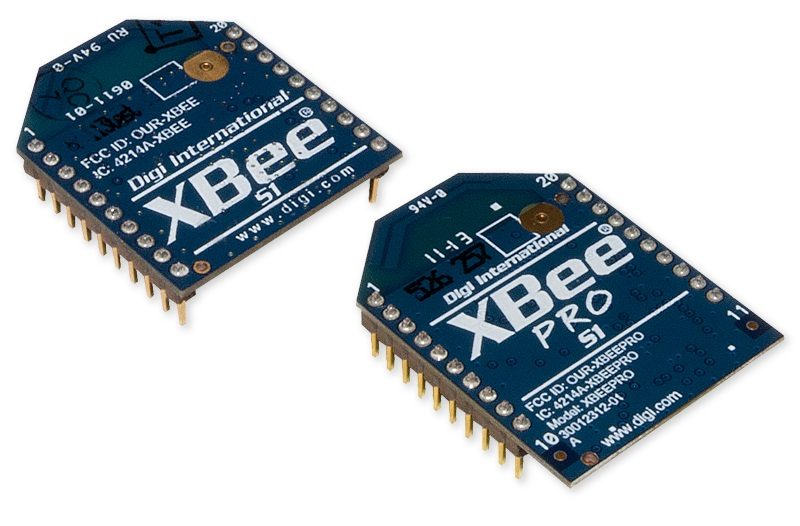
\includegraphics[width=0.95\textwidth]{figures/Xbee.jpg}
			\caption{Two Xbee radio modules\cite{Digi} } 
			\label{XbeeLook}
		\end{figure}
	\end{minipage}
	\hspace{0.03\linewidth}
	\begin{minipage}{0.45\linewidth}
		\begin{figure}[H]
			\centering
			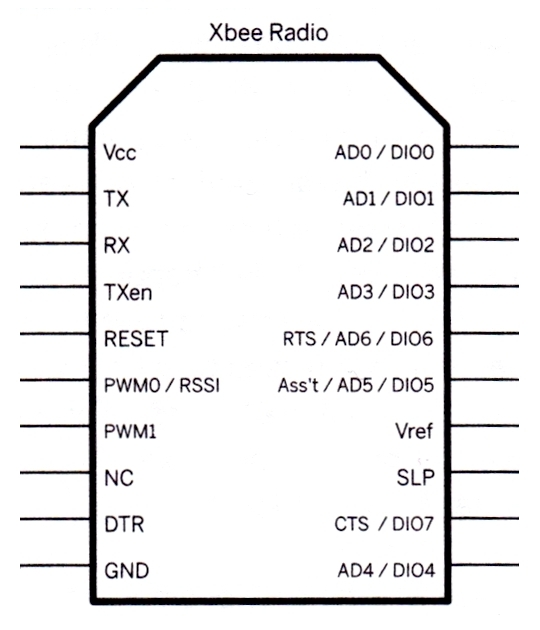
\includegraphics[width=0.95\textwidth]{figures/XbeeIO.jpg}
			\caption{Pinout of an Xbee radio module\cite{jeromeabel}} 
			\label{Xbeepinout}
		\end{figure}
	\end{minipage}
\end{minipage}


The Xbee modules communicate through an UART connection (with TX and RX pins)\cite{Xbee}. Since the Arduino has three UART connections, plus the one used to program the Arduino, the Xbee can be connected. The software code for the GoT system is implemented in C\# (see in \secref{GoTDescription}) and the computer running has serial ports that can ensure the connection between the software and the Xbee. Therefore, this solution can be used for a wireless connection between the GoT system and the Arduino.

To run the Xbee modules, a \si{3,3\ V} power line, a ground line, and a \si{3,3\ V} logic UART are needed\cite{Xbee}. The modules have a transfer speed of up to \si{115,2 kbit/s} and can reach up to \si{100 m} indoor and \si{300 m} outdoor. It transmits at a \si{2,4 GHz} frequency with \si{1 mV} (\si{0 dBm}) and can receive downto \si{-96 dBm}\cite{Xbee}. The Xbee is already ready for communication, with the lower levels of communication, the physical and data link layers, being already implemented. With only two devices, a lightweight combination of transport layer can be added to the protocol directly on top of the data link layer, to add more error handling and create the transmitted packet.



%%%%%%%%%%%%%%%%%%%%%%%%%%%%%%%%%%%%%%%%%%%%%%%%%%%%%

\subsection{Angular sensor}
The angular sensor is used in the feedback for the control system.

The servomotor needs to receive commands every \si{30\ ms}, \cite{futaba}. The measurements from the angular sensor will therefore also be sampled at this frequency. 

\begin{flalign}
	\eq{Sampling\ frequency}{\frac{1}{0.0030}  = 33.3 \si{Hz}}
\end{flalign}

The requirements for the angular sensor are:
\begin{itemize}
\item It is possible to control it by utilizing the Arduino Mega.
\item Able to achieve a sampling frequency at 33.3 \si{Hz}.
\end{itemize}

\subsubsection{HMC5883L}
Sparkfun's "9 degrees of freedom" board\cite{Sparkfun9D0F} comprises a magnetometer integrated circuit, the HMC5883L. A magnetometer will be used as the angular sensor, since it can be set up as a compass and give out a angle compared to north. 

\begin{figure}[H]
	\centering
	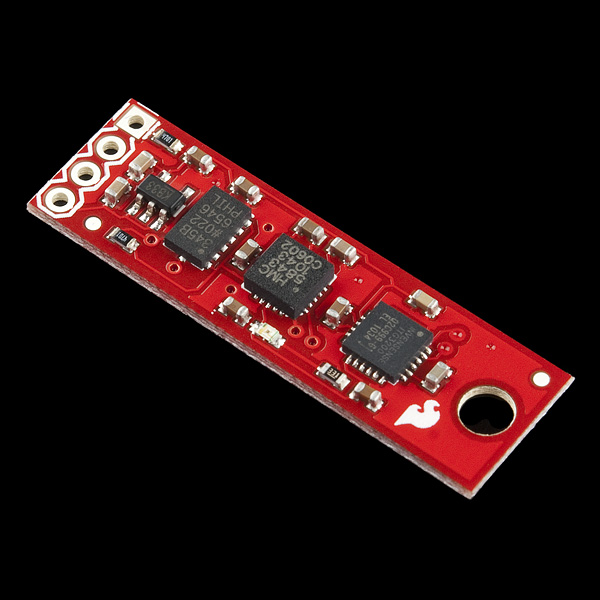
\includegraphics[width=0.50\textwidth]{figures/NineDegree.jpg}
		\caption{Sparksfun's "9 degrees of freedom" sensor stick\cite{Sparkfun9D0F} } 
	\label{NineDegree}
\end{figure}

The "9 degrees of freedom" sensor stick, see \figref{NineDegree}, will be used in the project. Beside the magnetometer, there are also a accelerometer and a gyroscope on the board, but these will not be used. The "9 degrees of freedom" sensor stick is designed to be used with a microcontroller and comes with software example for the Arduino platform. It needs an  \si{I^2C} bus to communicate with the Arduino, which has that kind of interface.

%%%%%%%%%%%%%%%%%%%%%%%%%%%%%%%%%%%%%%%%%%%%%%%%%%%%%

\subsection{Power monitor}
The power monitor is used to give a feedback to the system about the level of power in the battery pack.

Requirements for the power monitor:
\begin{itemize}
\item Can be monitored by the Arduino Mega.
\item Measuring the battery pack voltage output downto \si{6\ V}, \secref{sec:Vehicledescription}.
\end{itemize}

\subsubsection{Voltage divider}
A voltage divider is an electronic circuit, that divides the input voltage with a constant depending on the values of the resistors used in the circuit, see \figref{VoltDivFig}.

\begin{figure}[h!]
\centering
\begin{circuitikz}
\draw (0,0)
to[V,v=$V_{in}$] (0,2)
to[short] (2,2)
to[R=$R_1$] (2,0)
to[R=$R_2$] (2,-2)
to[short] (0,-2)
to[short] (0,0);
\draw (2,-2) 
to[short] node[ground] {} (2,-3);
\draw (2,0)
to[short] (3,0)
to[short,l=$V_{out}$] (4,0);
\end{circuitikz}
\caption{Standard voltage divider} 
\label{VoltDivFig}
\end{figure}

The output of the voltage divider can be found with \eqref{VoltageDivider}. 
%
\begin{flalign}
\eq{V_{out}}{\frac{R_2}{R_1 + R_2} \cdot V_{in}}\unit{V} 
\label{VoltageDivider}
\end{flalign}
\hspace{6mm} Where:\\
\begin{tabular}{p{1cm}lll}
& \si{V_{in}} & is the battery pack voltage &\unitWh{V} \\
& \si{R_1, R_2} & are two calculated resistors &\unitWh{\Omega}\\
& \si{V_{out}} & is the measured output voltage &\unitWh{V}
\end{tabular}
%
The input voltage is set to be the battery pack and the output is measured though an analogue pin on the Arduino. The analogue pin on the Arduino can measure from \si{0\ V} to \si{5\ V} with a resolution of \si{10\ bits}. This gives 1023 steps from 0 to 5 volts and each step is \si{4,9\ mV}. The size of each step and the range for the measuring is multiplied with the inverse constant, that comes from the two resistor, so it is possible to make the range go over \si{5\ V}. 

A voltage divider is used in this project, as it can be scaled to the interval that it has to measure. The voltage divider will be connected to an analogue pin on the Arduino, which will make the measurement from the output of the voltage divider.

From the preanalysis it has been possible to choose hardware which needs to be utilized. After having chosen the different hardware components for the prototype, the different components have to be implemented in the system.
%%%%%%%%%%%%%%%%%%%%%%%%%%%%%%%%%%%%%%%%%%%%%%%%%%%%%


%Pins on the arduino
%SD card (4 I/O)
%Xbee (1 TX and 1 RX)
%Hall (2 I/O)
%Angular (1 SDL and 1 SDA)
%Servo (1 PWM)
%Motor (1 PWM)
